\FloatBarrier
\section{The ANNNI-type Model}
\label{sec:annni}

We study a self-dual quantum spin chain that extends the transverse-field Ising model with \ac{NNN} interactions~\cite{alcaraz2016}. For spin-$1/2$ degrees of freedom, the Hamiltonian is
\begin{equation}
    H = - \sum_{i} \Big[ \sigma_i^z \sigma_{i+1}^z + \lambda\, \sigma_i^x
        \;+\; p\,\big( \sigma_i^z \sigma_{i+2}^z + \lambda\, \sigma_i^x \sigma_{i+1}^x \big) \Big],
    \label{eq:annni_H}
\end{equation}
where $\sigma^{x,z}$ are Pauli matrices, $\lambda$ is the transverse field, and $p$ controls the strength of the additional interactions. The $\sigma^x\sigma^x$ term preserves self-duality under the Kramers--Wannier transformation~\cite{alcaraz2016}, which fixes the critical point at $\lambda=1$. We work at this point throughout, so that the conformal predictions of Section~\ref{sec:cft} apply.

At $p=0$, Eq.~\eqref{eq:annni_H} reduces to the integrable transverse-field Ising chain. For $p>0$, a \ac{JW} transformation no longer maps the Hamiltonian to free fermions, and the model is therefore non-integrable. The origin of the fermionic interactions is detailed in Appendix~\ref{sec:annni:jw}.

\subsection{Equilibrium criticality and the central charge}
\label{sec:annni:equilibrium}

We restrict our equilibrium calculations to $0\le p\le1.5$, the range over which the model is known to remain critical and in the Ising universality class~\cite{alcaraz2016}. We verify the equilibrium universality class over this range using the ground-state entanglement. For a critical open chain of length $L$, \ac{CFT} predicts that the von Neumann entropy of a block of length $l$ scales as~\cite{holzhey1994,vidal2003,calabrese_cardy2004}
\begin{equation}
    S_{\mathrm{vN}}(l,L) = \frac{c}{6}\,W(l,L) + k,
    \label{eq:cft_obc}
\end{equation}
where $W$ is the chord variable of Eq.~\eqref{eq:chord} and $k$ is a non-universal constant. The von Neumann entropy is well suited to this calculation because \ac{DMRG} provides the full ground-state Schmidt spectrum directly, and also has weaker finite-size corrections than the higher-order R\'enyi entropies~\cite{cardy_calabrese2010,calabrese2010}.

For each value of $p$, we obtain the ground state of a chain with $N=400$ sites and evaluate the entropy across every bond. Equation~\eqref{eq:cft_obc} predicts a linear dependence on $W(l,L)$, so the entanglement profile of a single ground state provides an estimate of the central charge. We fit only the middle part of the chain, using the cuts satisfying $0.25L<l<0.75L$, where boundary corrections are smallest. The resulting profiles are shown in Figure~\ref{fig:cft_chord}.

\begin{figure}[H]
    \centering
    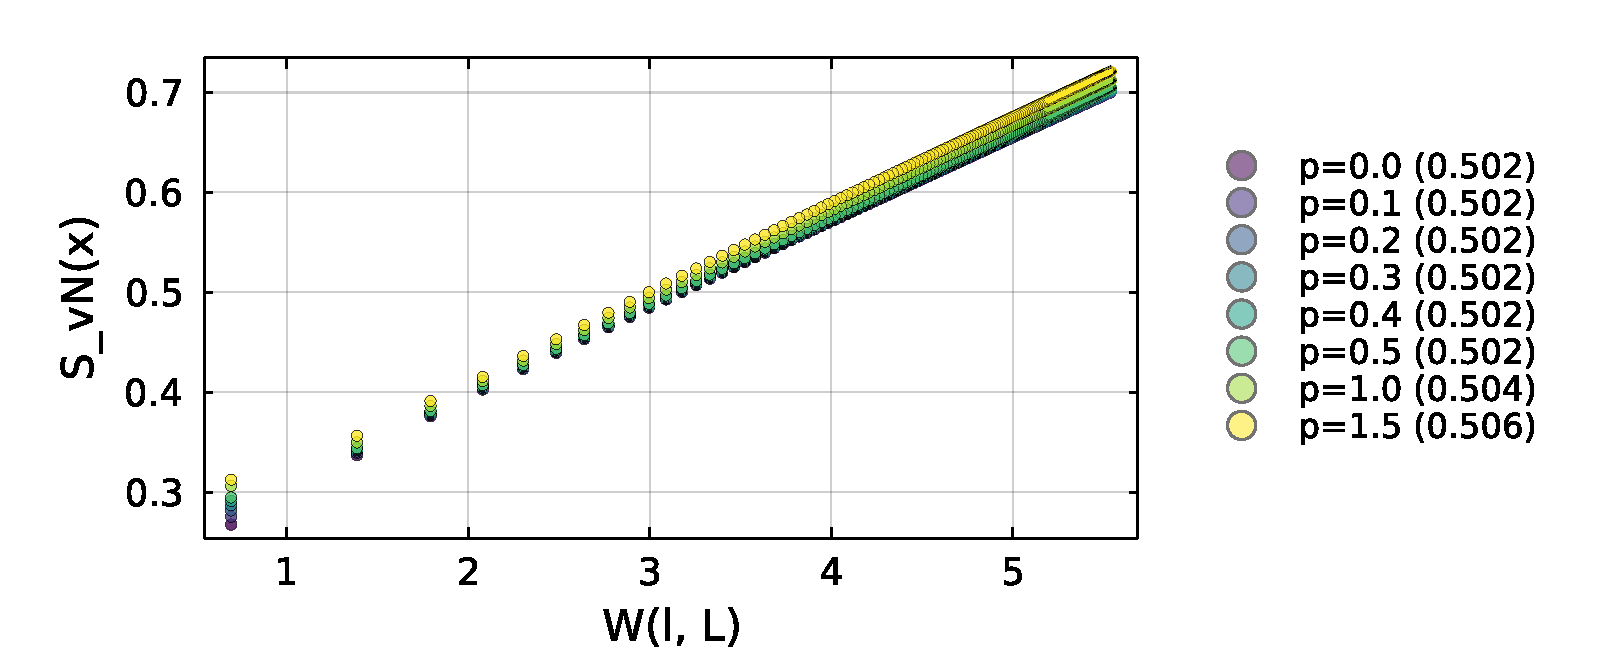
\includegraphics[width=0.80\textwidth]{imgs/cft_chord_equilibrium.pdf}
    \caption{\textbf{Effect of \ac{NNN} interactions on the equilibrium central charge.} Ground-state entanglement profiles at $\lambda=1$ and $N=400$, for the eight couplings $p=0$ to $1.5$, plotted against the chord variable $W$ of Eq.~\eqref{eq:chord}, which is smallest for cuts near the chain ends. Circles are the entropies at each cut; the solid line through each profile is the fit over the middle half of the chain, whose central charge is given in the legend. The linear dependence on $W$ gives a value close to the Ising $c=1/2$ at every $p$, with a small common offset from finite-size corrections.}
    \label{fig:cft_chord}
\end{figure}

The profiles follow the conformal scaling law at every coupling, and the fitted central charge barely changes with $p$. Its small common offset from the exact value $c=1/2$ is consistent with residual finite-size corrections to Eq.~\eqref{eq:cft_obc}, since a similar offset is already present at the exactly solvable point $p=0$. The additional interactions therefore do not change the universality class over the range considered. This agrees with previous finite-size scaling studies of the same chain~\cite{alcaraz2016}, and with an independent determination that extracts the conformal data directly from the lattice Hamiltonian~\cite{milsted2017}.

The profiles separate at small $W$, where the cuts lie closest to the open boundaries. Equation~\eqref{eq:cft_obc} is less accurate in this region because the boundaries introduce corrections that depend on the microscopic interactions and therefore on $p$, which is why these cuts are left out of the fit. Towards the centre of the chain, these boundary effects weaken and the profiles converge towards the common linear behaviour predicted by \ac{CFT}. Appendix~\ref{app:fss} gives an independent estimate from the finite-size scaling of the mid-chain entropy and a cross-check using the R\'enyi-2 entropy.

\subsection{Sound velocity}
\label{sec:annni:velocity}

The \ac{NNN} interaction changes how fast excitations travel along the chain. At an Ising-class critical point, the low-energy dispersion is linear, $\omega(k)=v|k|$, so the sound velocity $v$ fixes the relativistic scale of the continuum theory~\cite{difrancesco1997}. It enters three of the four predictions of Section~\ref{sec:cft} explicitly, because those predictions are written in terms of lengths on the conformal strip and $v$ is what turns an evolution time into such a length~\cite{cardy1984,blote_cardy_nightingale1986}; in the entropy profile it only shifts the non-universal offset. The velocity must therefore be measured independently before the predictions can be compared with the dynamical data. At $p=0$ the chain is a free-fermion model with the exact dispersion $\omega(k)=4|\sin(k/2)|$, hence $v=2$~\cite{pfeuty1970}; for $p>0$ we determine $v$ numerically.

We extract $v(p)$ from the equilibrium dispersion of the same chain, Eq.~\eqref{eq:annni_H} at $\lambda=1$, placed on rings of $N$ sites with periodic boundary conditions and diagonalised exactly. The momenta on a ring are quantised, so the slope follows from the energy of the lowest excitation carrying the smallest non-zero momentum~\cite{alcaraz2016}. Because exact diagonalisation is restricted to small rings, we repeat this at five lengths and extrapolate with a $1/N^2$ dependence, a form fixed empirically at the integrable point where the answer is known (Appendix~\ref{app:velocity}). This procedure reproduces the exact result at $p=0$ and is then applied at each non-zero coupling $p$.

The velocity grows steadily from $2.000$ at $p=0$ to $10.799$ at $p=1.5$, as shown in Figure~\ref{fig:velocity}. Although the velocity is non-universal, it is fixed by the model; we determine it from the equilibrium spectrum and use the independently extrapolated value at each coupling in all subsequent conversions. Appendix~\ref{app:velocity} describes the dispersion calculation, extrapolation and validation in detail.

\begin{figure}[htbp]
    \centering
    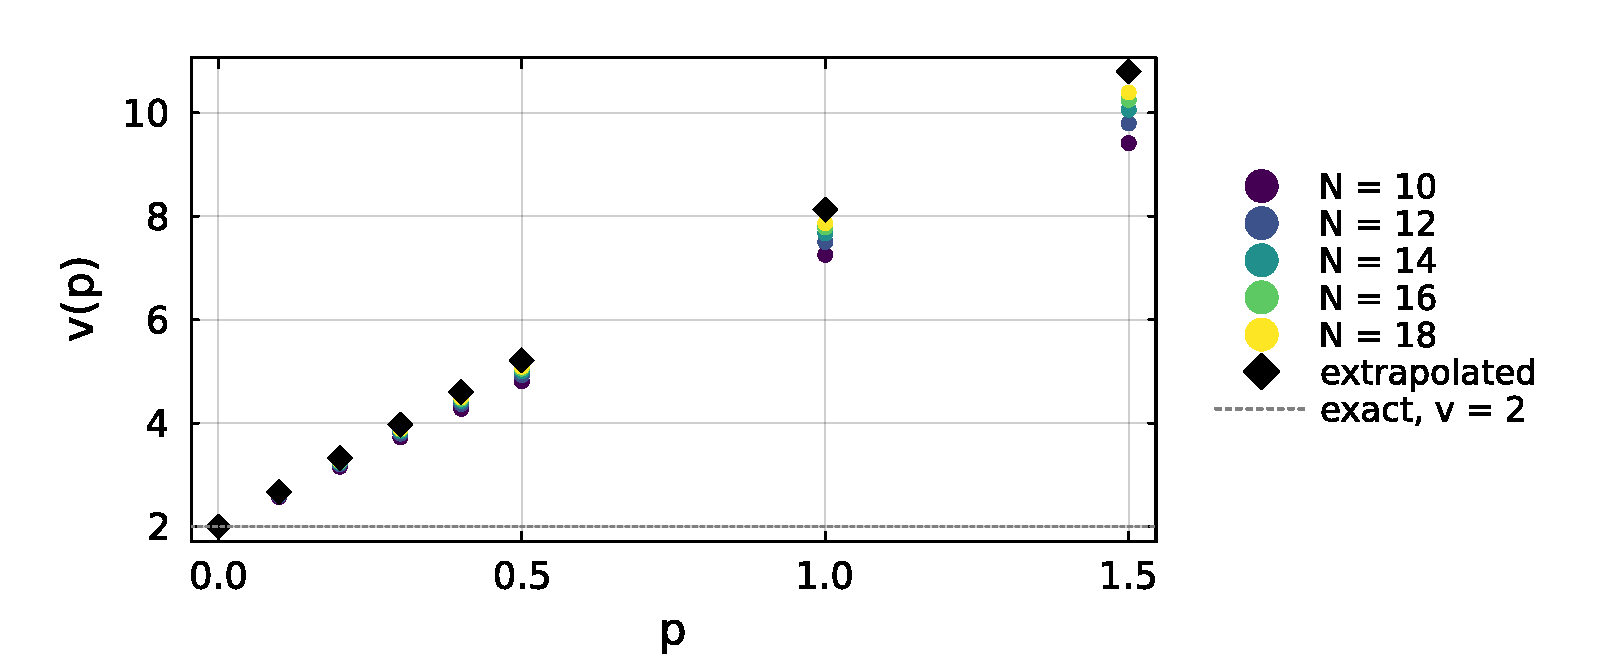
\includegraphics[width=0.80\textwidth]{imgs/velocity_vs_p.pdf}
    \caption{\textbf{The sound velocity grows with the \ac{NNN} coupling.} $v(p)$ at $\lambda=1$, from the equilibrium dispersion of periodic rings of $N=10$ to $18$ sites (coloured circles), together with the values extrapolated to the thermodynamic limit (black diamonds), which are the ones used throughout. The dotted line marks the exact Ising value $v=2$ at $p=0$.}
    \label{fig:velocity}
\end{figure}
